\begin{frame}{Cross-section as function of $c_{i}$}
\begin{columns}
\column{0.5\textwidth}    
\begin{figure}
    \centering
    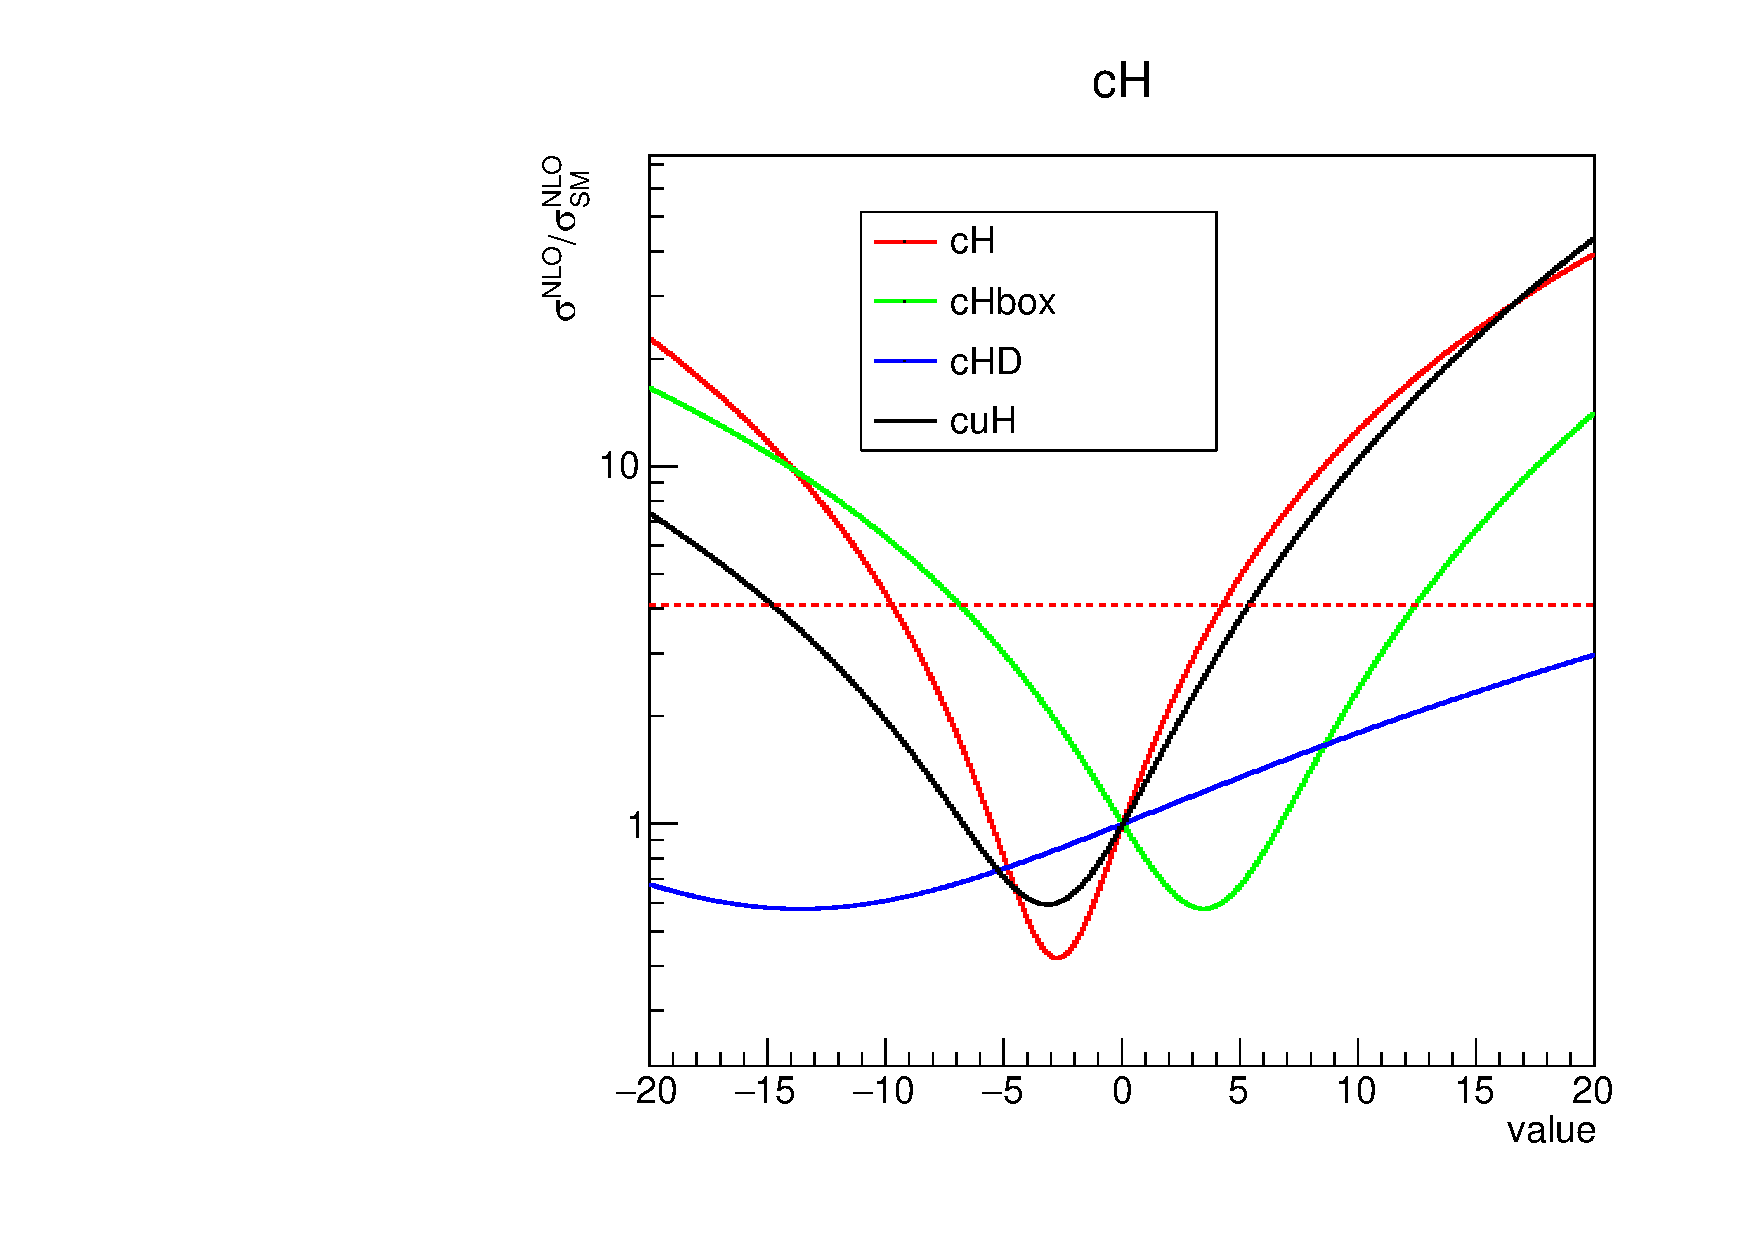
\includegraphics[width=1.\textwidth]{BackUp/Part5/Img/Xsec_NLO_with_SM.pdf}
\end{figure}
\column{0.5\textwidth}
\begin{figure}
    \centering
    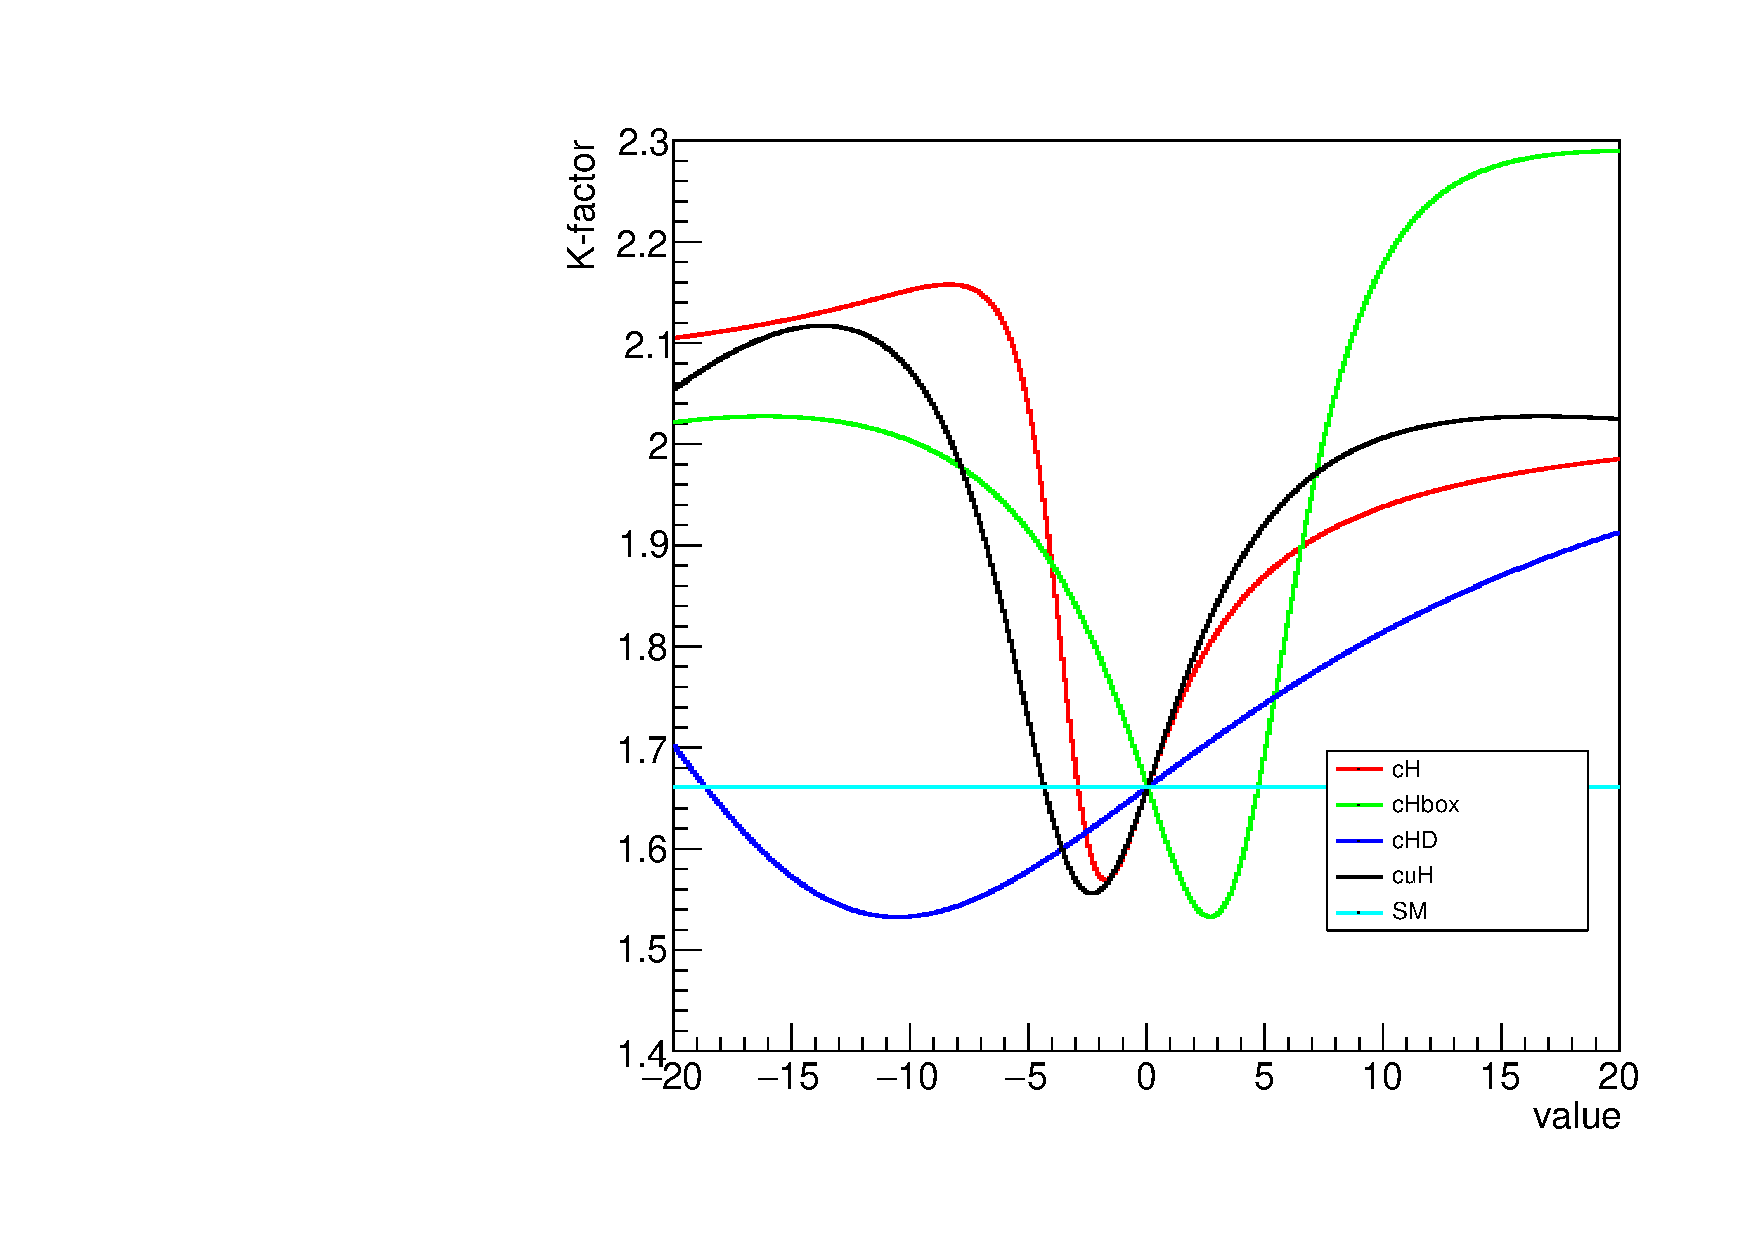
\includegraphics[width=1.\textwidth]{BackUp/Part5/Img/k_factor_with_SM.pdf}
\end{figure}
\end{columns}
\end{frame}

\begin{frame}{Linear vs quadratic : $m_{HH}$ distribution}
\begin{columns}
\column{0.5\textwidth}    

Interference
\begin{figure}
    \centering
    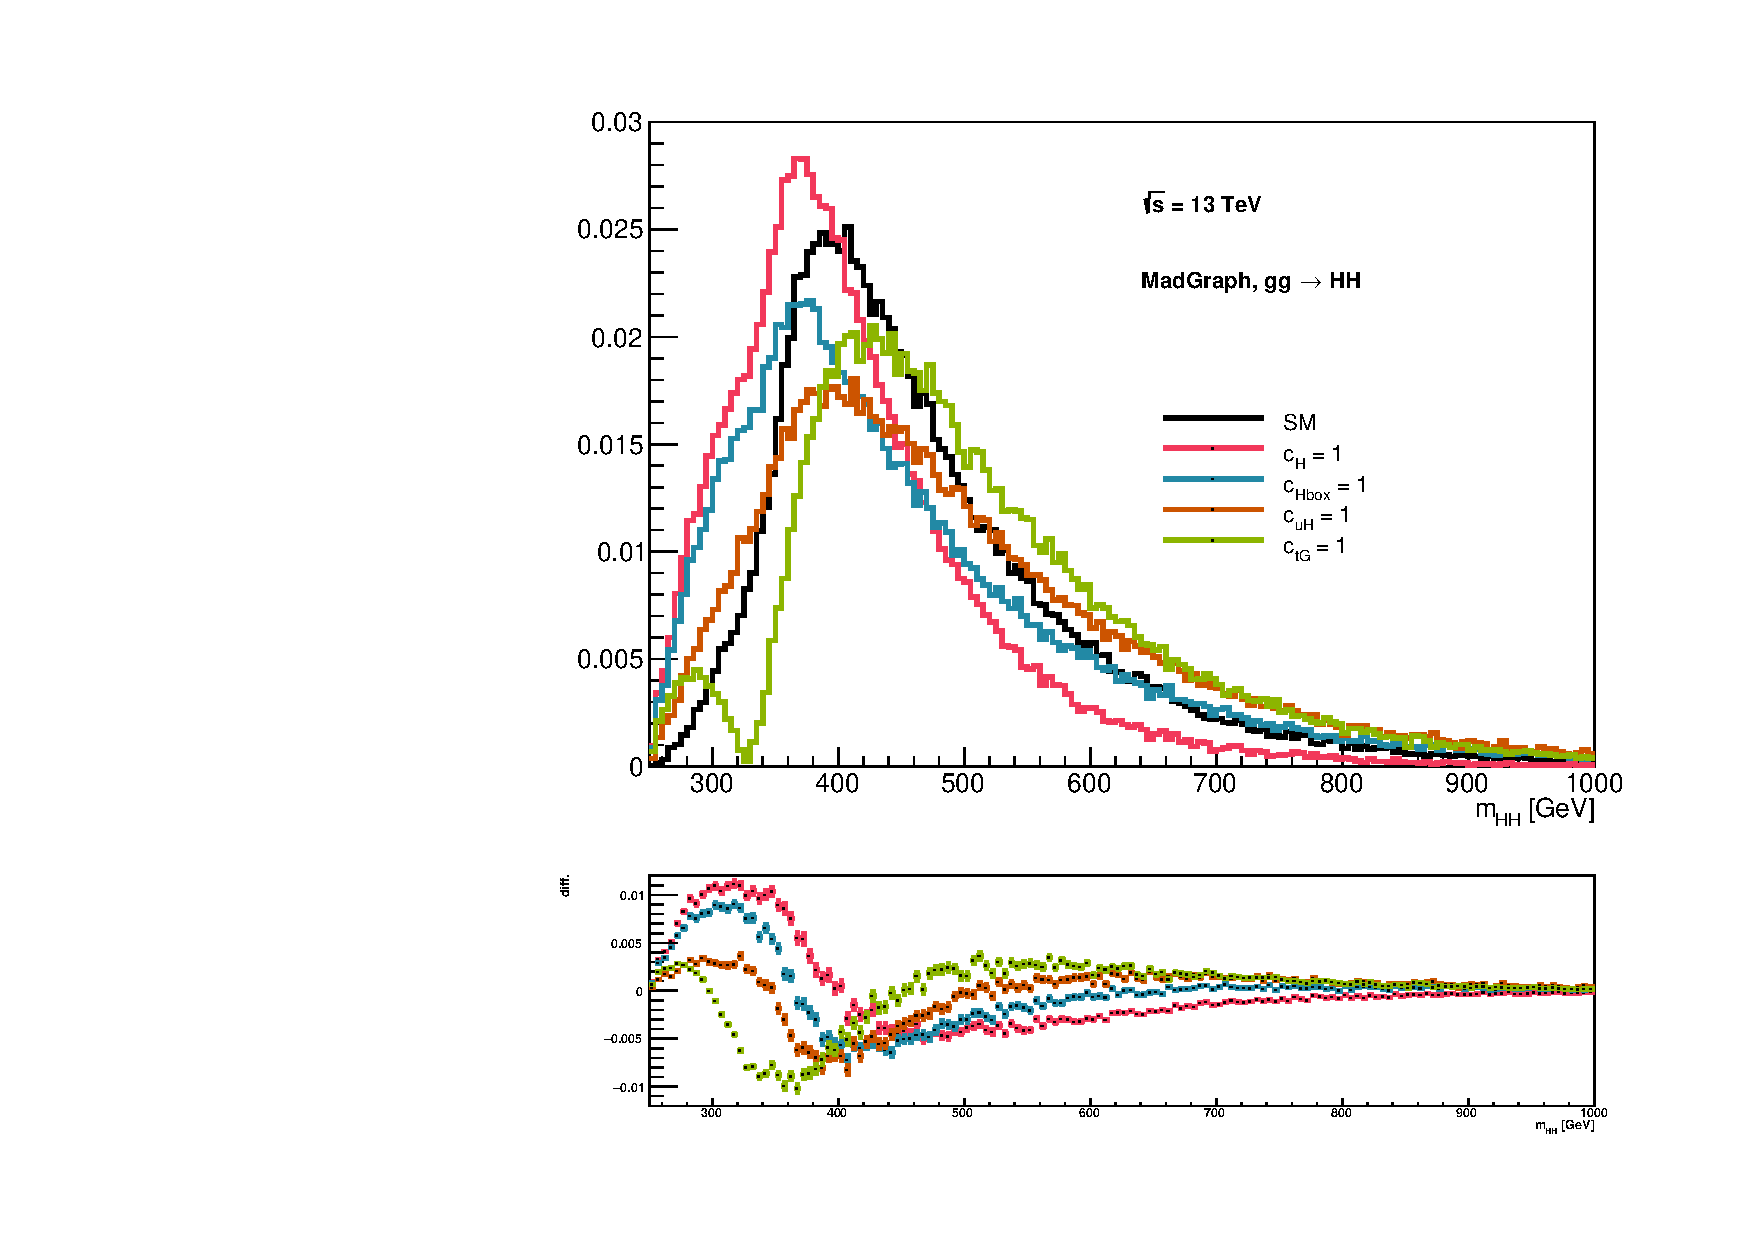
\includegraphics[width=1.\textwidth]{Part5/Img/EFT_suplot.pdf}
\end{figure}
    
\column{0.5\textwidth}

pure BSM
\begin{figure}
    \centering
    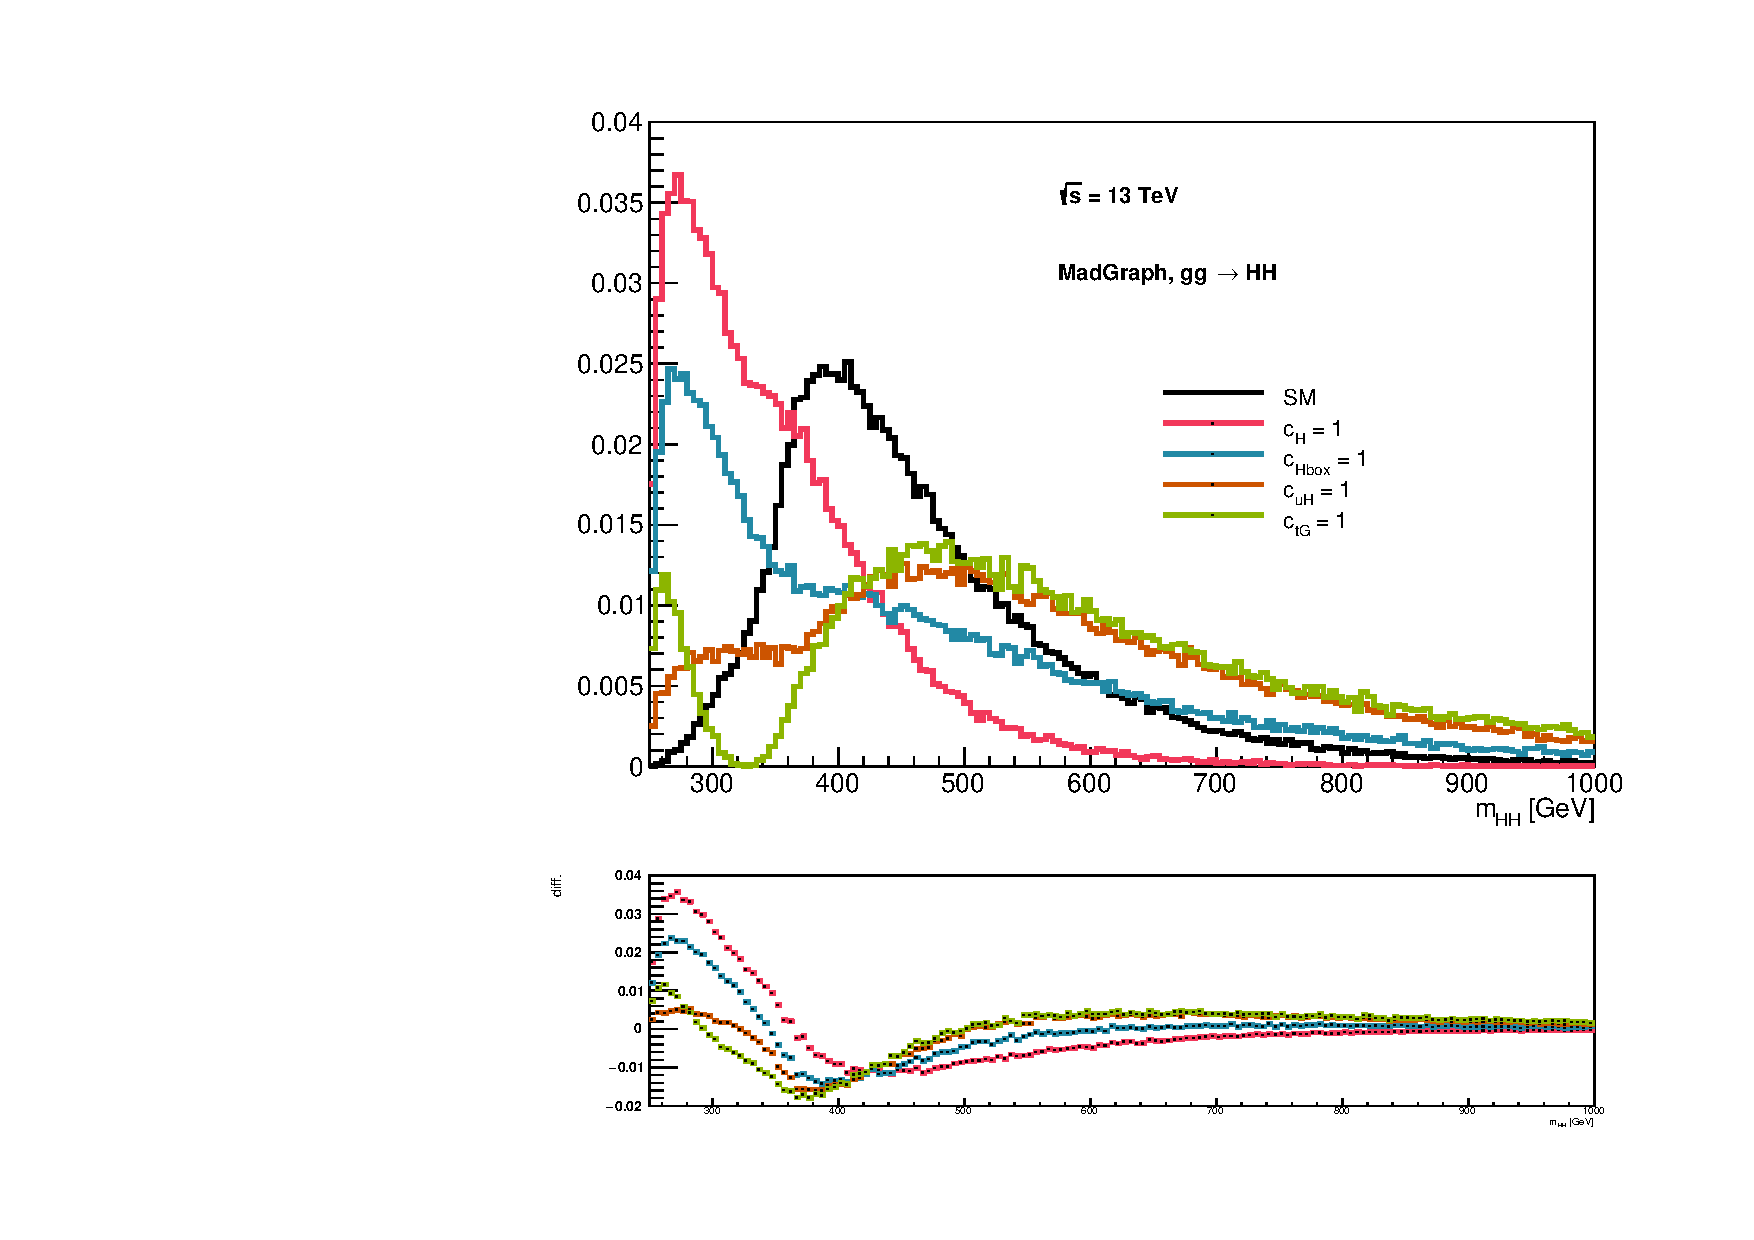
\includegraphics[width=1.\textwidth]{BackUp/Part5/Img/EFT_suplot_Quad.pdf}
\end{figure}

\end{columns}
\end{frame}

\begin{frame}{Linear vs quadratic : Cross-section}
\begin{columns}
\column{0.5\textwidth}    

Interference
\begin{figure}
    \centering
    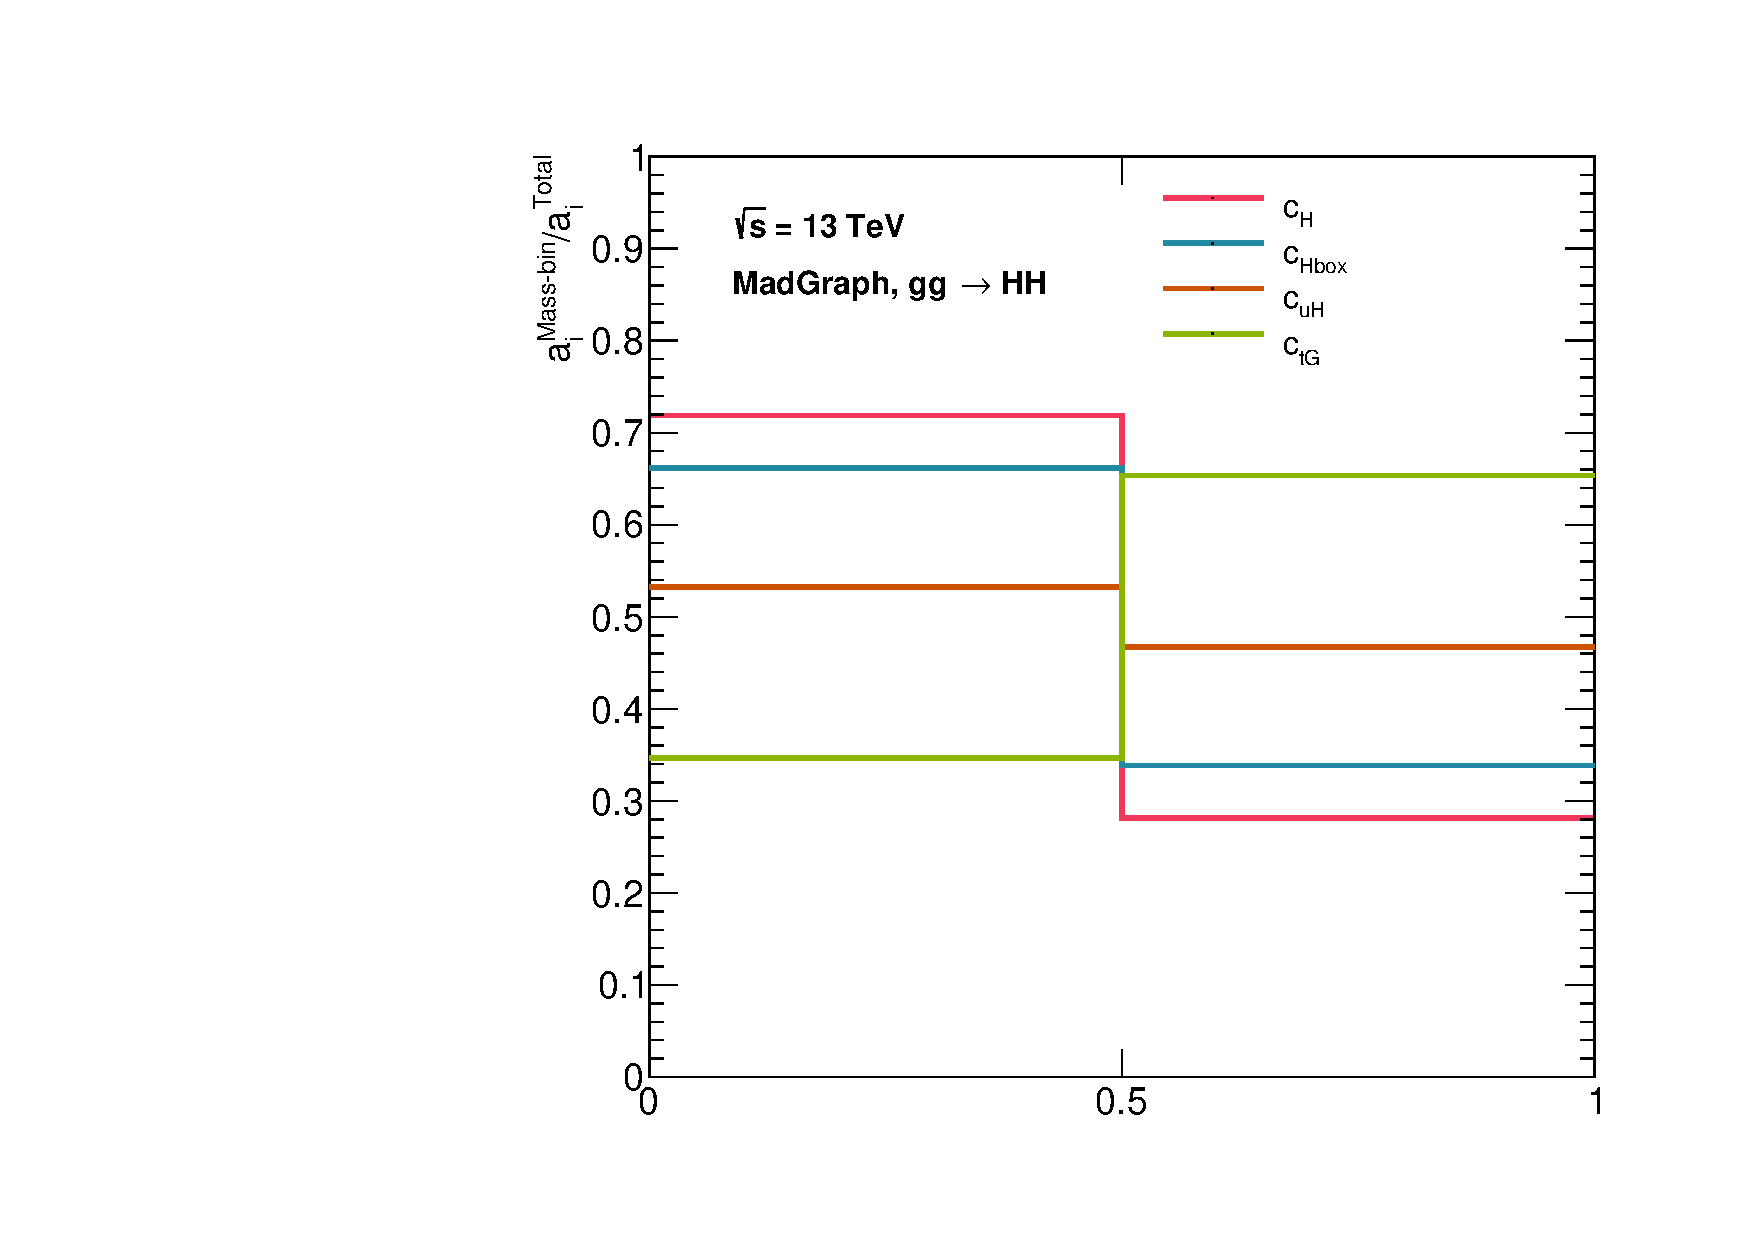
\includegraphics[width=1.\textwidth]{Part5/Img/a_i_total.pdf}
\end{figure}
    
\column{0.5\textwidth}

pure BSM
\begin{figure}
    \centering
    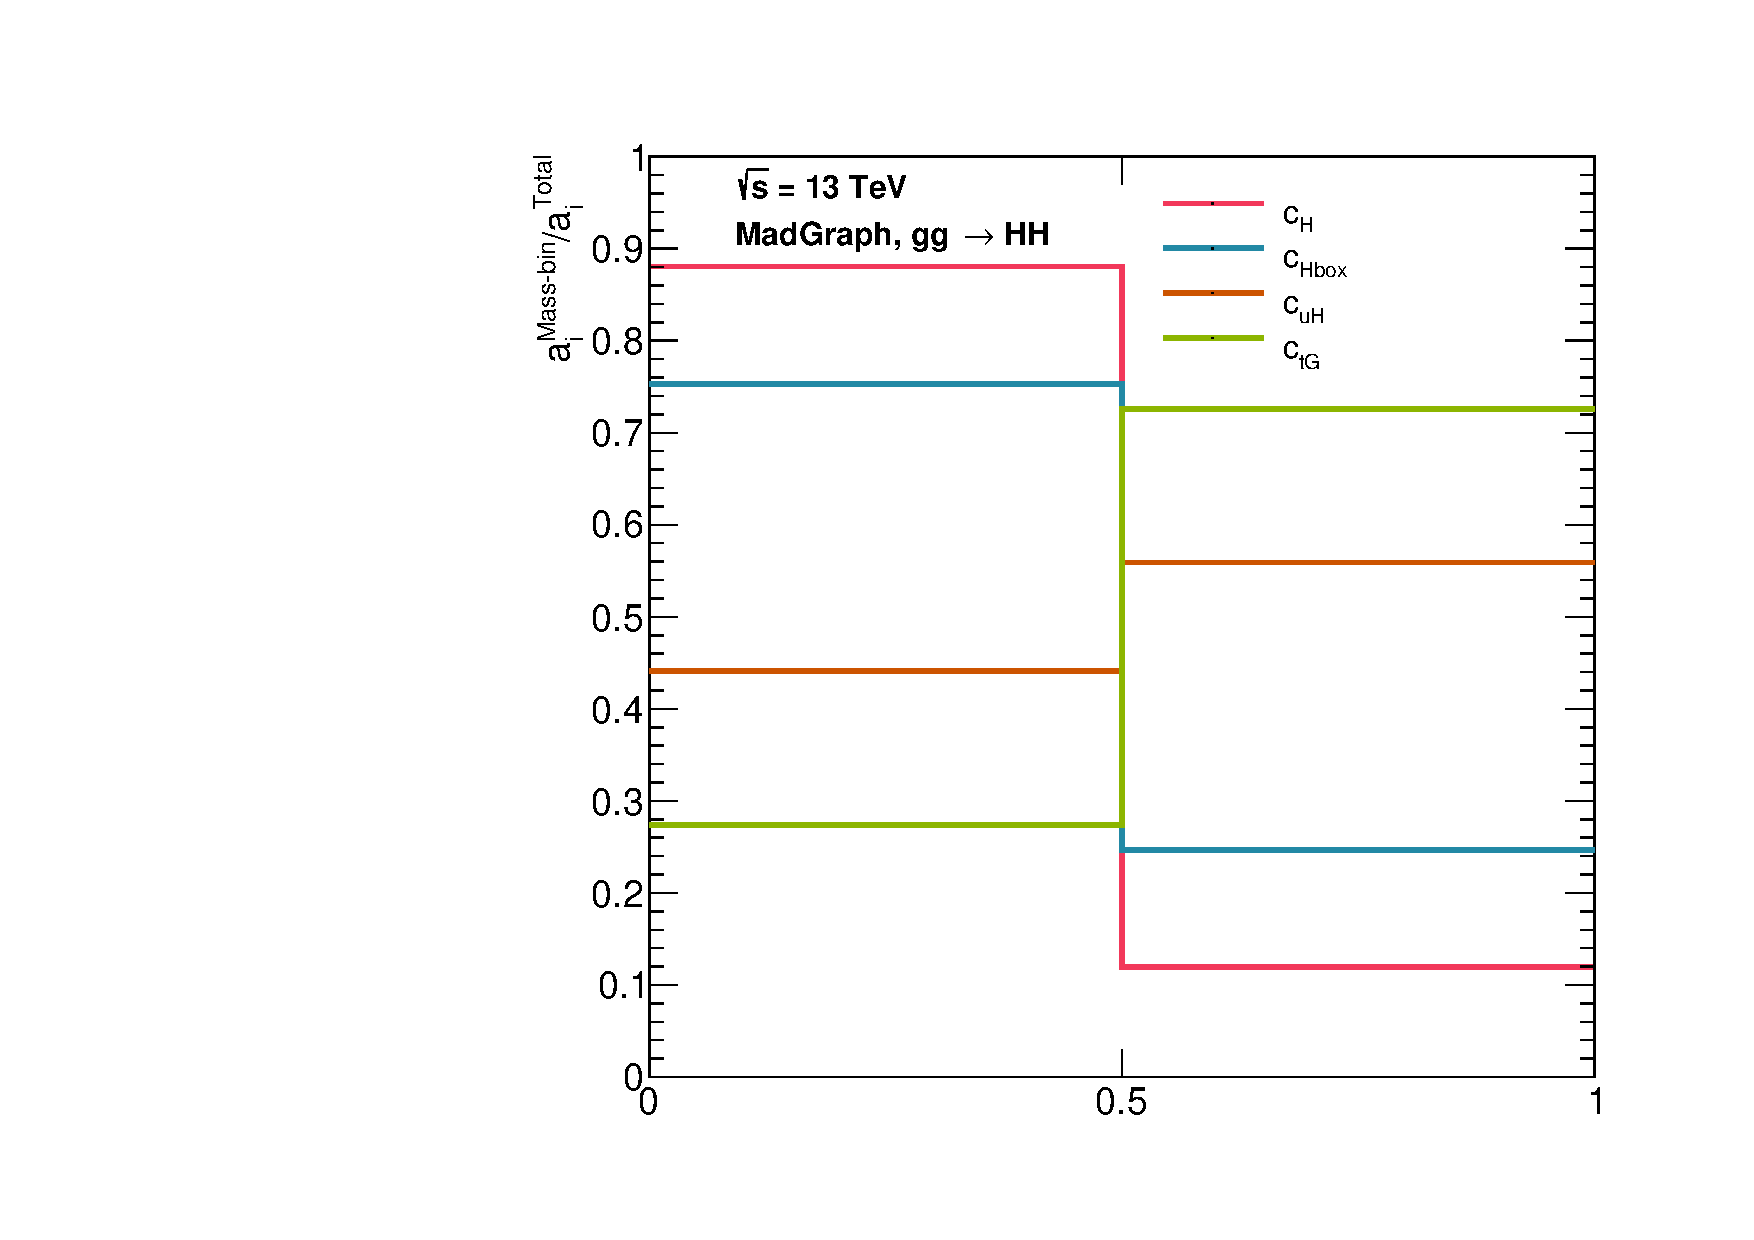
\includegraphics[width=1.\textwidth]{BackUp/Part5/Img/a_i_total_Quad.pdf}
\end{figure}

\end{columns}
\end{frame}

\begin{frame}{Cross-section parameterization}
\begin{itemize}
    \item ggF HH events simulated using MadGraph events generator + SMEFTatNLO feynrules model (using NLO card).
    \item Each term (linear and quadratic) is generated separately: 
    
    \begin{table}[]
        \centering
        \begin{tabular}{lc}
        \hline\hline
            Command & term \\
        \hline    
            generate p p $>$ h h  QED=2 QCD=2 NP=2 [QCD] & SM only \\ 
            generate p p $>$ h h NP=2 QCD=2 QED=2 NP$^2$==2 [QCD] & Interference \\
            generate p p $>$ h h NP=2 QCD=2 QED=2 NP$^2$==4 [QCD]  & BSM only \\
        \hline\hline    
        \end{tabular}
    \end{table}
    \item 4 EFT variations are generated for each operator, $c_{i} = \pm1, \pm2$
    \item $\frac{\sigma}{\sigma_{SM}}$ fitted in each mass region (High mass and Low mass) using
    \item Cross-term effect considered by generating an additional $c_{i,j} = 1$ BSM sample and subtract individual quadratic contribution. 
\end{itemize}    
\end{frame}

\begin{frame}{$c_{H}$ parameterization}
\begin{columns}
\column{0.5\textwidth}
\begin{figure}
    \centering
    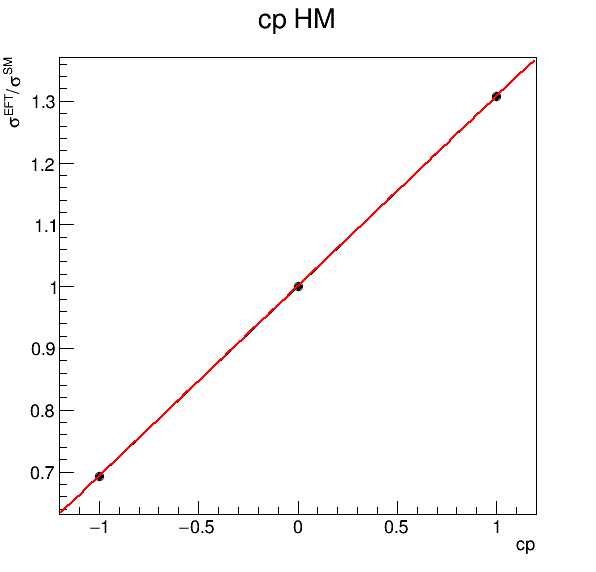
\includegraphics[width=1.\textwidth]{BackUp/Part5/Img/cp_MG_Fit_HM.png}
\end{figure}
\column{0.5\textwidth}
\begin{figure}
    \centering
    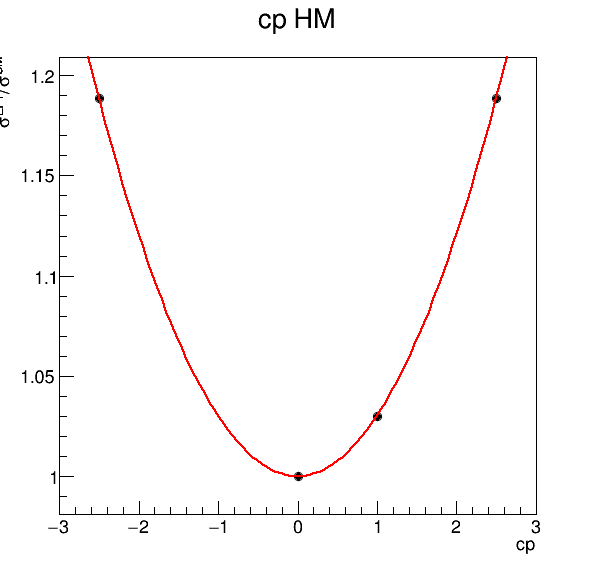
\includegraphics[width=1.\textwidth]{BackUp/Part5/Img/cp_MG_Fit_Quad_HM.png}
\end{figure}
\end{columns}

\end{frame}

\begin{frame}{Parametrization}
\begin{table}[]
    \begin{tabular}{ll}
    \hline\hline
    Region  & $\sigma/\sigma_{SM}$ \\
    \hline
    High mass &  - 0.19 $\cdot$ $c_{H\square}$ + 0.02 $\cdot$ $c_{H\square}^2$  + \textcolor{HHred}{0.31 $\cdot$ $c_{H}$}\\
    & + 0.03 $\cdot$ $c_{H}^2$ + 0.24 $\cdot$ $c_{uH}$ + 0.03 $\cdot$ $c_{uH}^2$ \\
    & - \textcolor{HHred}{0.30 $\cdot$ $c_{tG}$} + 0.05 $\cdot$ $c_{tG}^2$ - 0.04 $\cdot$ $c_{H}$ $\cdot$ $c_{H\square}$ \\
   & + 0.04 $\cdot$ $c_{H}$ $\cdot$ $c_{uH}$ - 0.06 $\cdot$ $c_{H}$ $\cdot$ $c_{tG}$ \\
   & - 0.05 $\cdot$ $c_{H\square}$ $\cdot$ $c_{uH}$ + 0.04 $\cdot$ $c_{H\square}$ $\cdot$ $c_{tG}$ \\
   & - 0.06 $\cdot$ $c_{uH}$ $\cdot$ $c_{tG}$ \\ 
   \hline
    Low mass &
    - 0.38 $\cdot$ $c_{H\square}$ + 0.05 $\cdot$ $c_{H\square}^2$ + \textcolor{HHturquoise_d}{0.79 $\cdot$ $c_{H}$} \\
  & +  0.22 $\cdot$ $c_{H}^2$ + 0.28 $\cdot$ $c_{uH}$ +  0.02 $\cdot$ $c_{uH}^2$ \\
  & - \textcolor{HHturquoise_d}{0.16 $\cdot$ $c_{tG}$} + 0.02 $\cdot$ $c_{tG}^2$  - 0.21 $\cdot$ $c_{H}$ $\cdot$ $c_{H\square}$ \\
  & + 0.14 $\cdot$ $c_{H}$ $\cdot$ $c_{uH}$ + 0.09 $\cdot$ $c_{H}$ $\cdot$ $c_{tG}$ \\
  & - 0.07 $\cdot$ $c_{H\square}$ $\cdot$ $c_{uH}$ - 0.03 $\cdot$ $c_{H\square}$ $\cdot$ $c_{tG}$ \\
  & + 0.03 $\cdot$ $c_{uH}$ $\cdot$ $c_{tG}$ \\
  \hline\hline
    \end{tabular}
\end{table}    
\end{frame}

\begin{frame}{likelihood scans}
\begin{columns}
\column{0.5\textwidth}
\begin{figure}
    \centering
    \subfloat{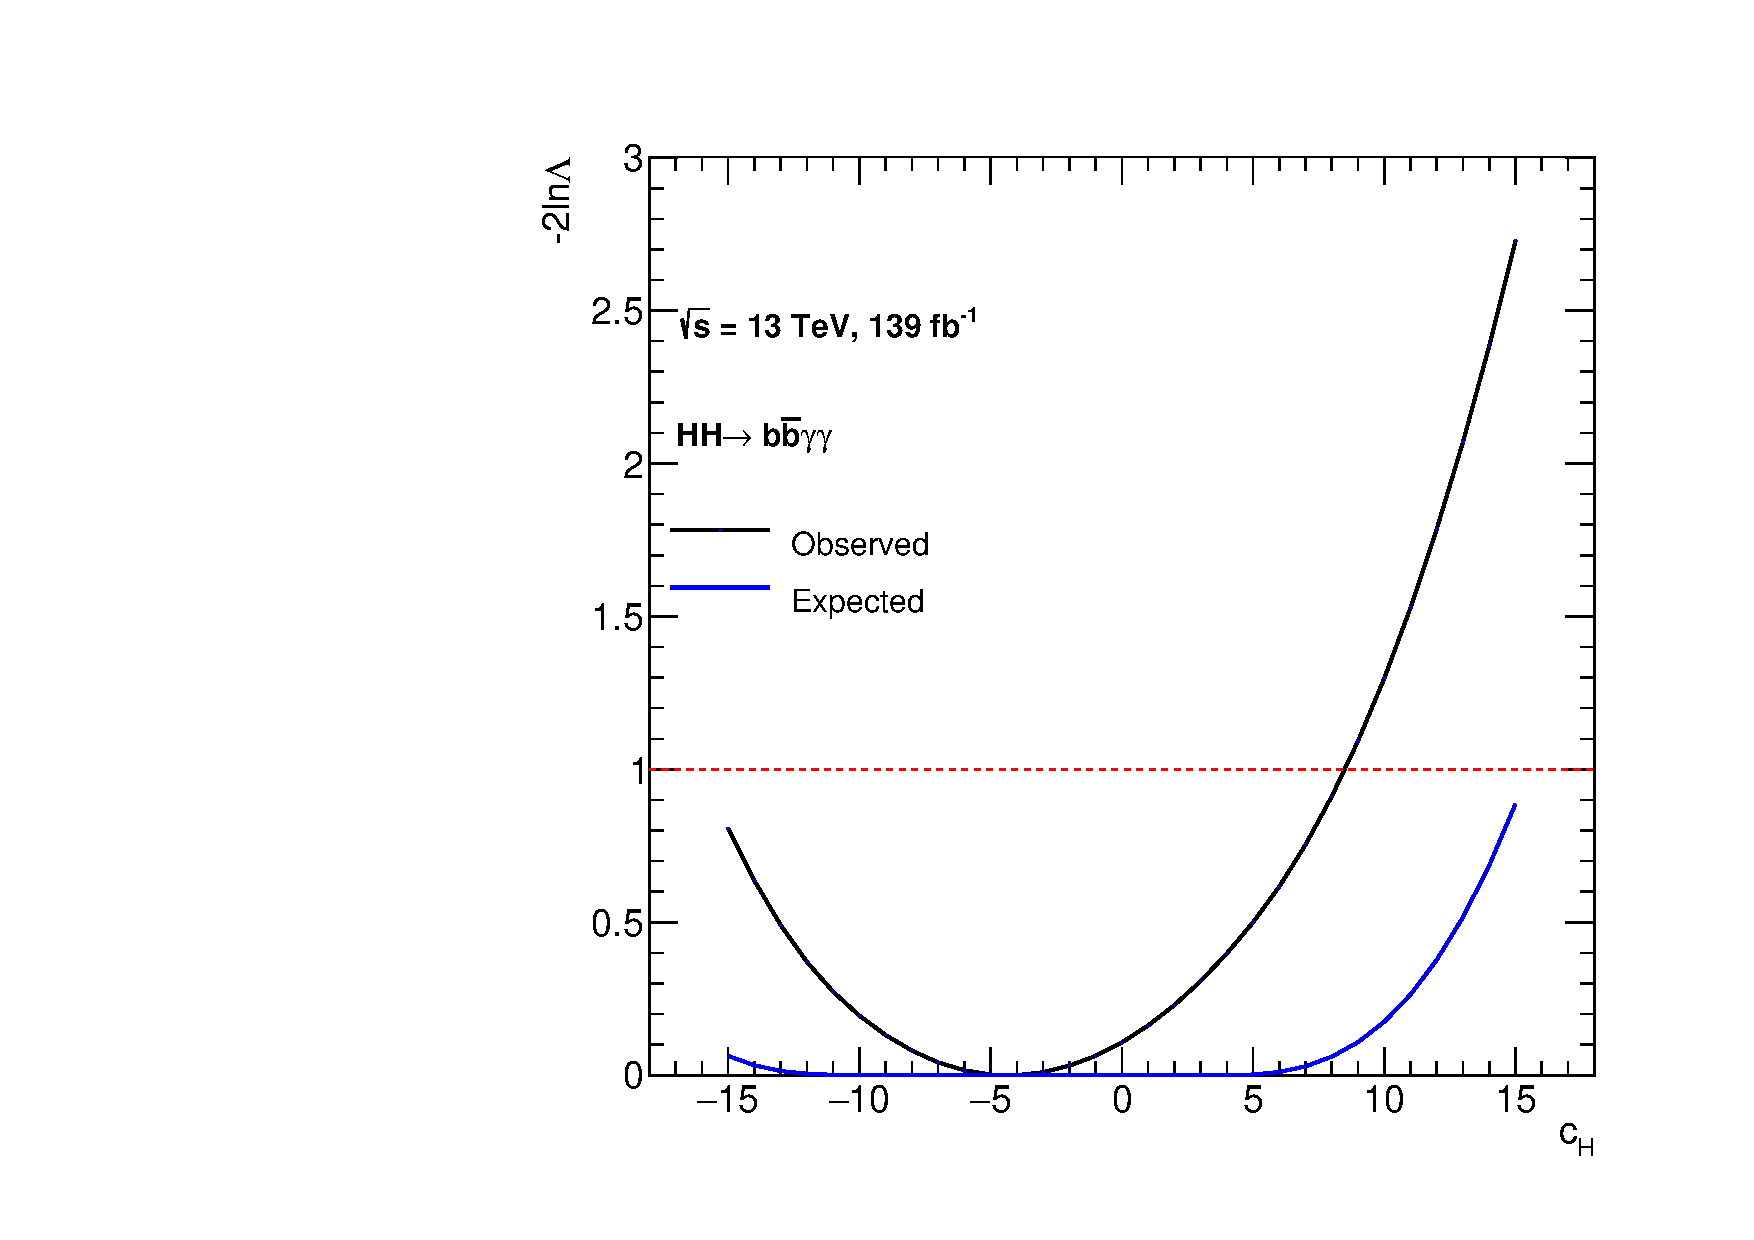
\includegraphics[width=0.5\textwidth]{BackUp/Part5/Img/subplot_NEW_cH_Observed_Expected_1_cHkin_MG.pdf}}\\
    \subfloat{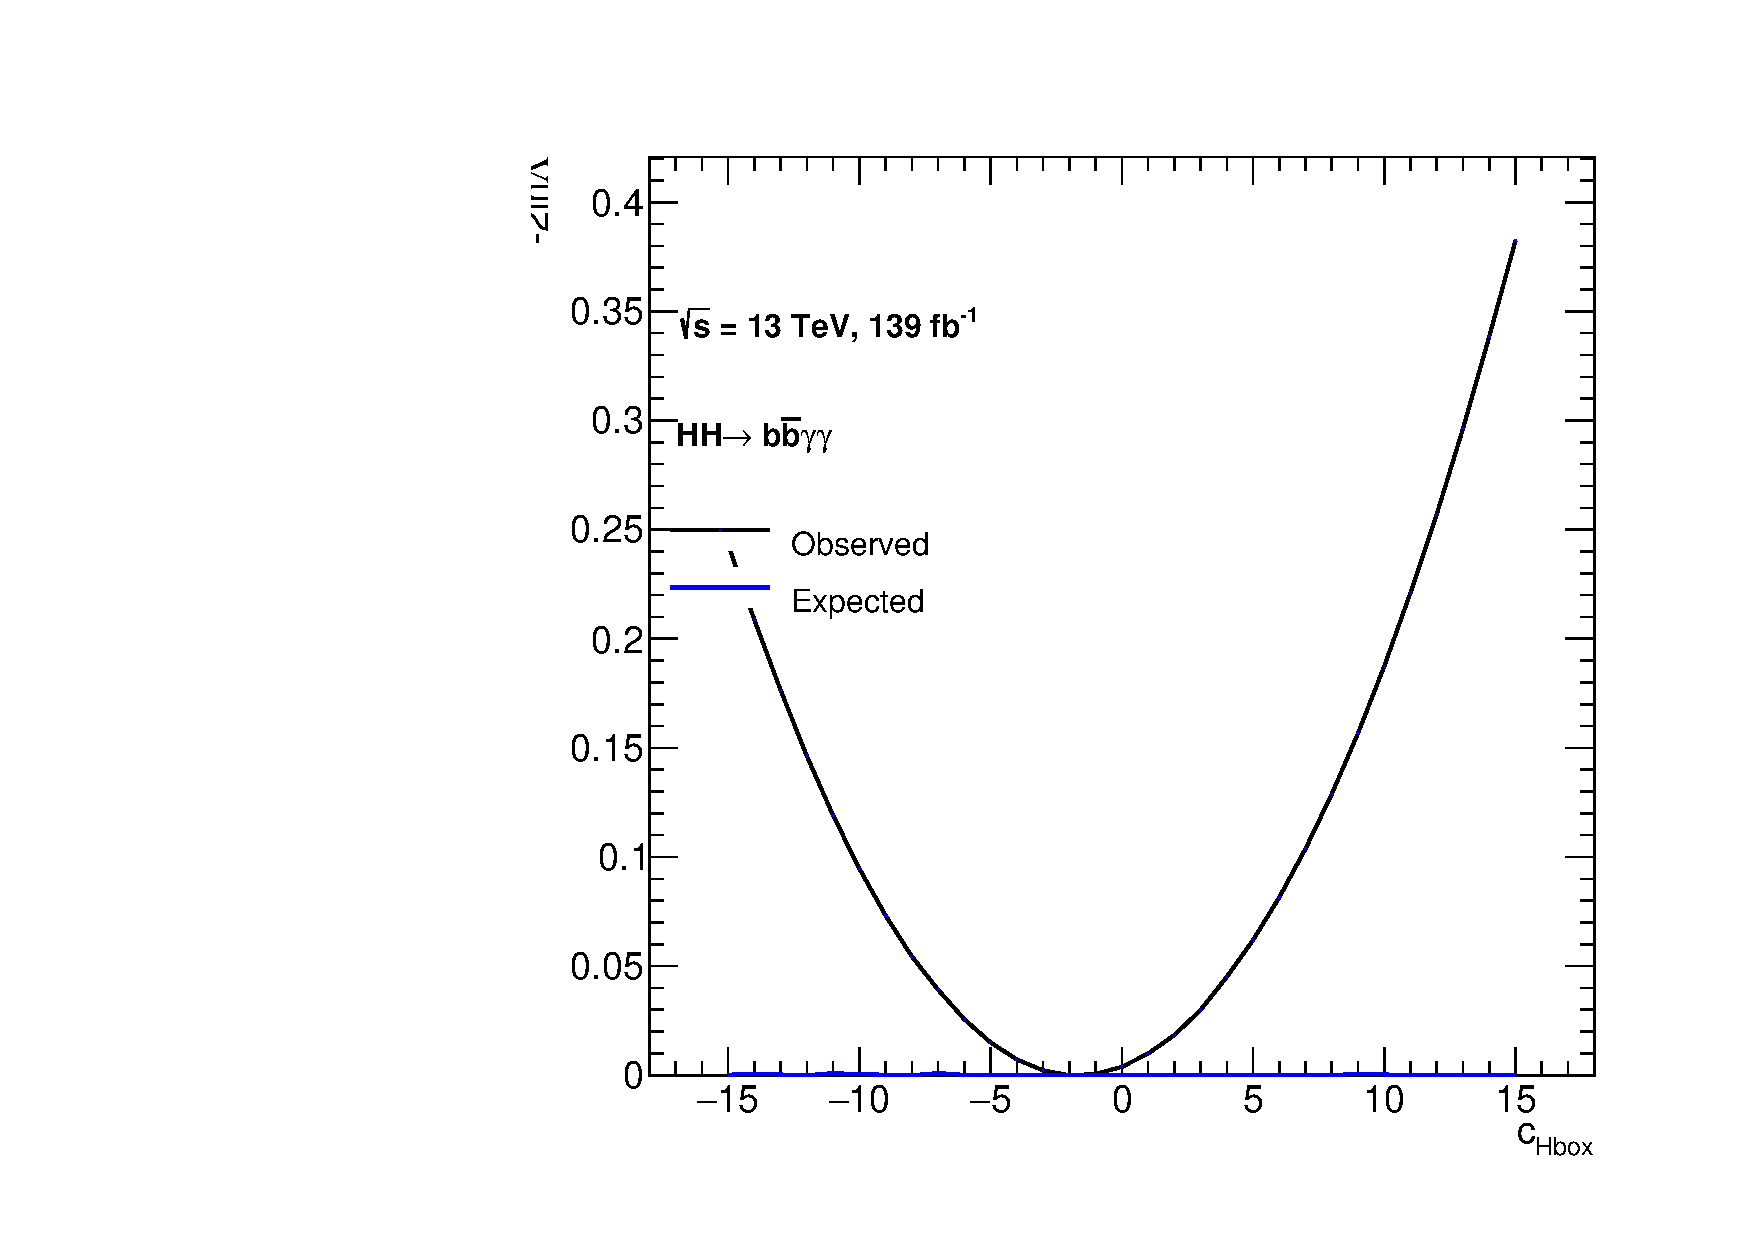
\includegraphics[width=0.5\textwidth]{BackUp/Part5/Img/subplot_NEW_cHkin_Observed_Expected_1_cHkin_MG.pdf}}
\end{figure}

\column{0.5\textwidth}
\begin{figure}
    \centering
    \subfloat{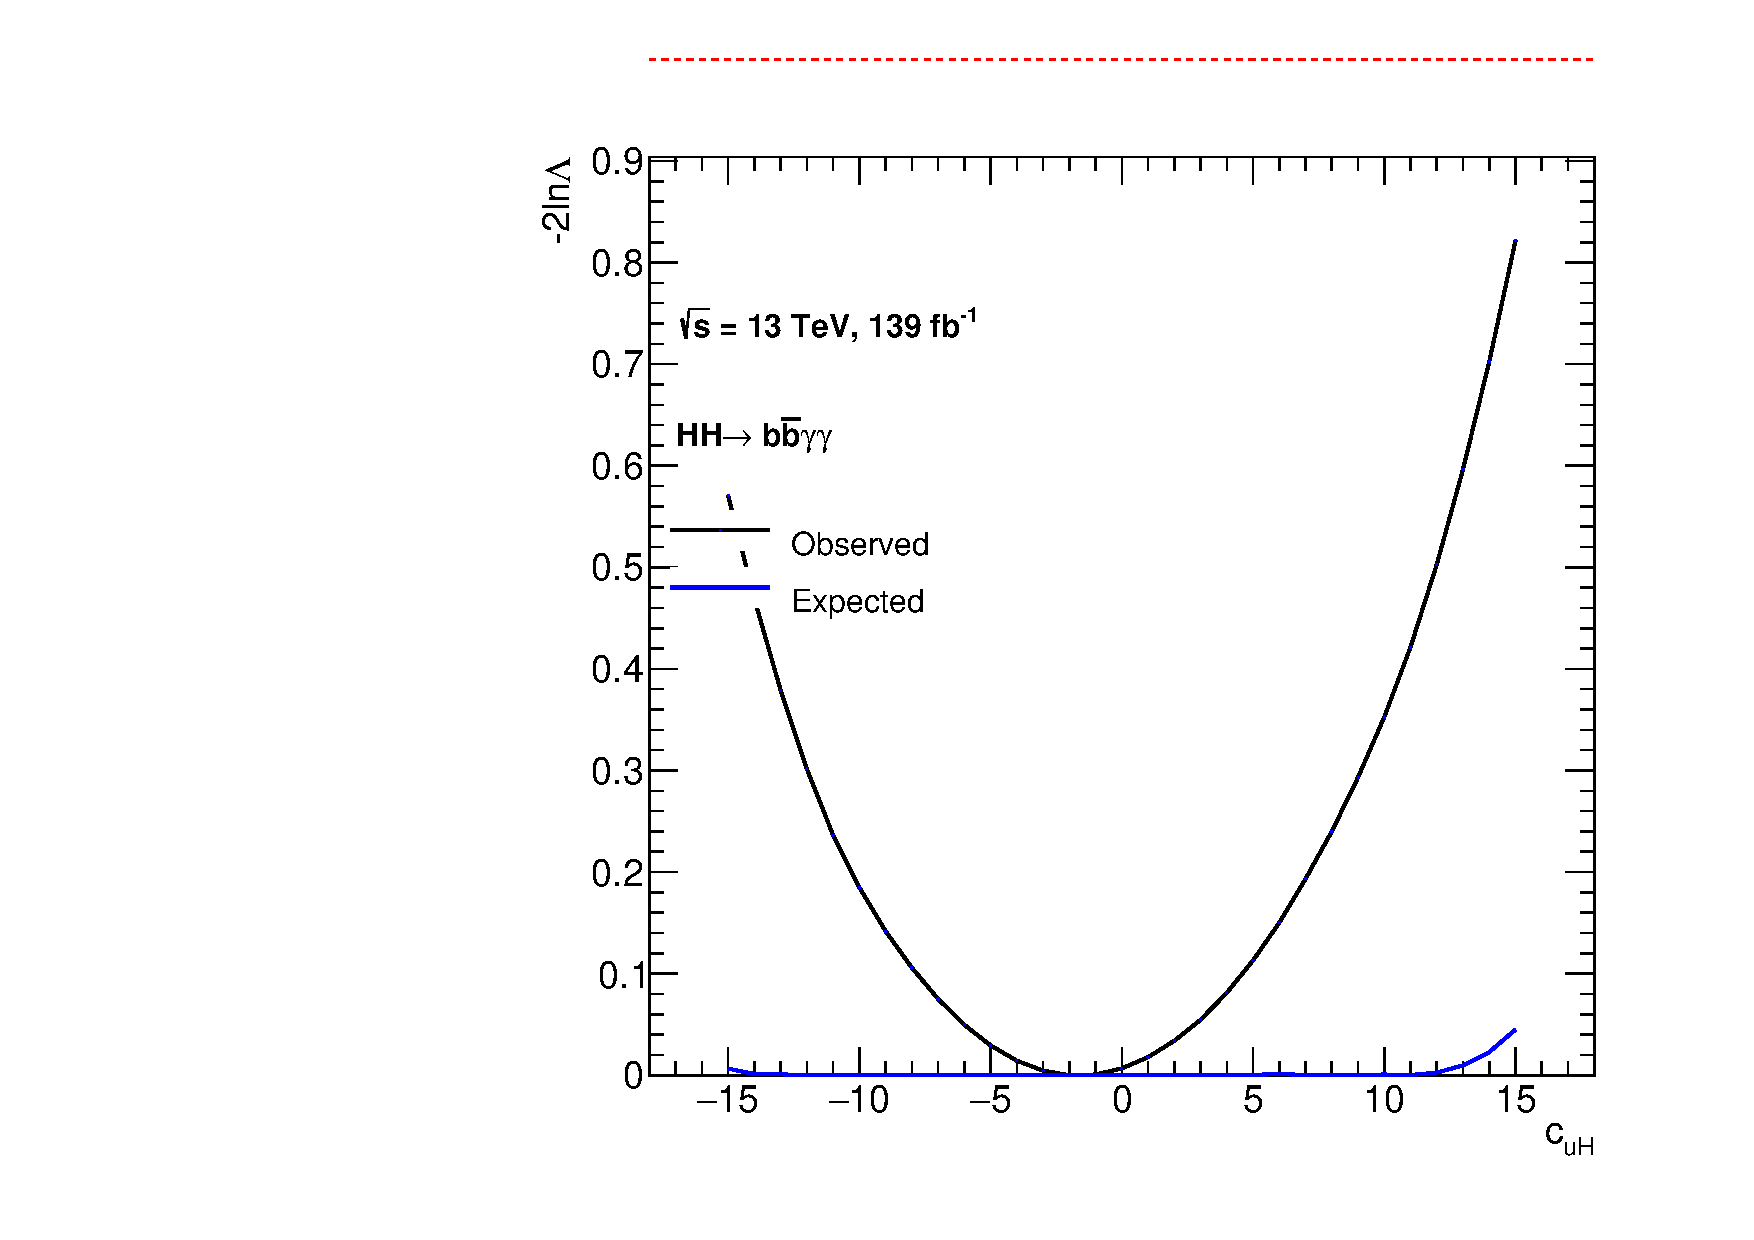
\includegraphics[width=0.5\textwidth]{BackUp/Part5/Img/subplot_NEW_cuH_Observed_Expected_1_cHkin_MG.pdf}}\\
    \subfloat{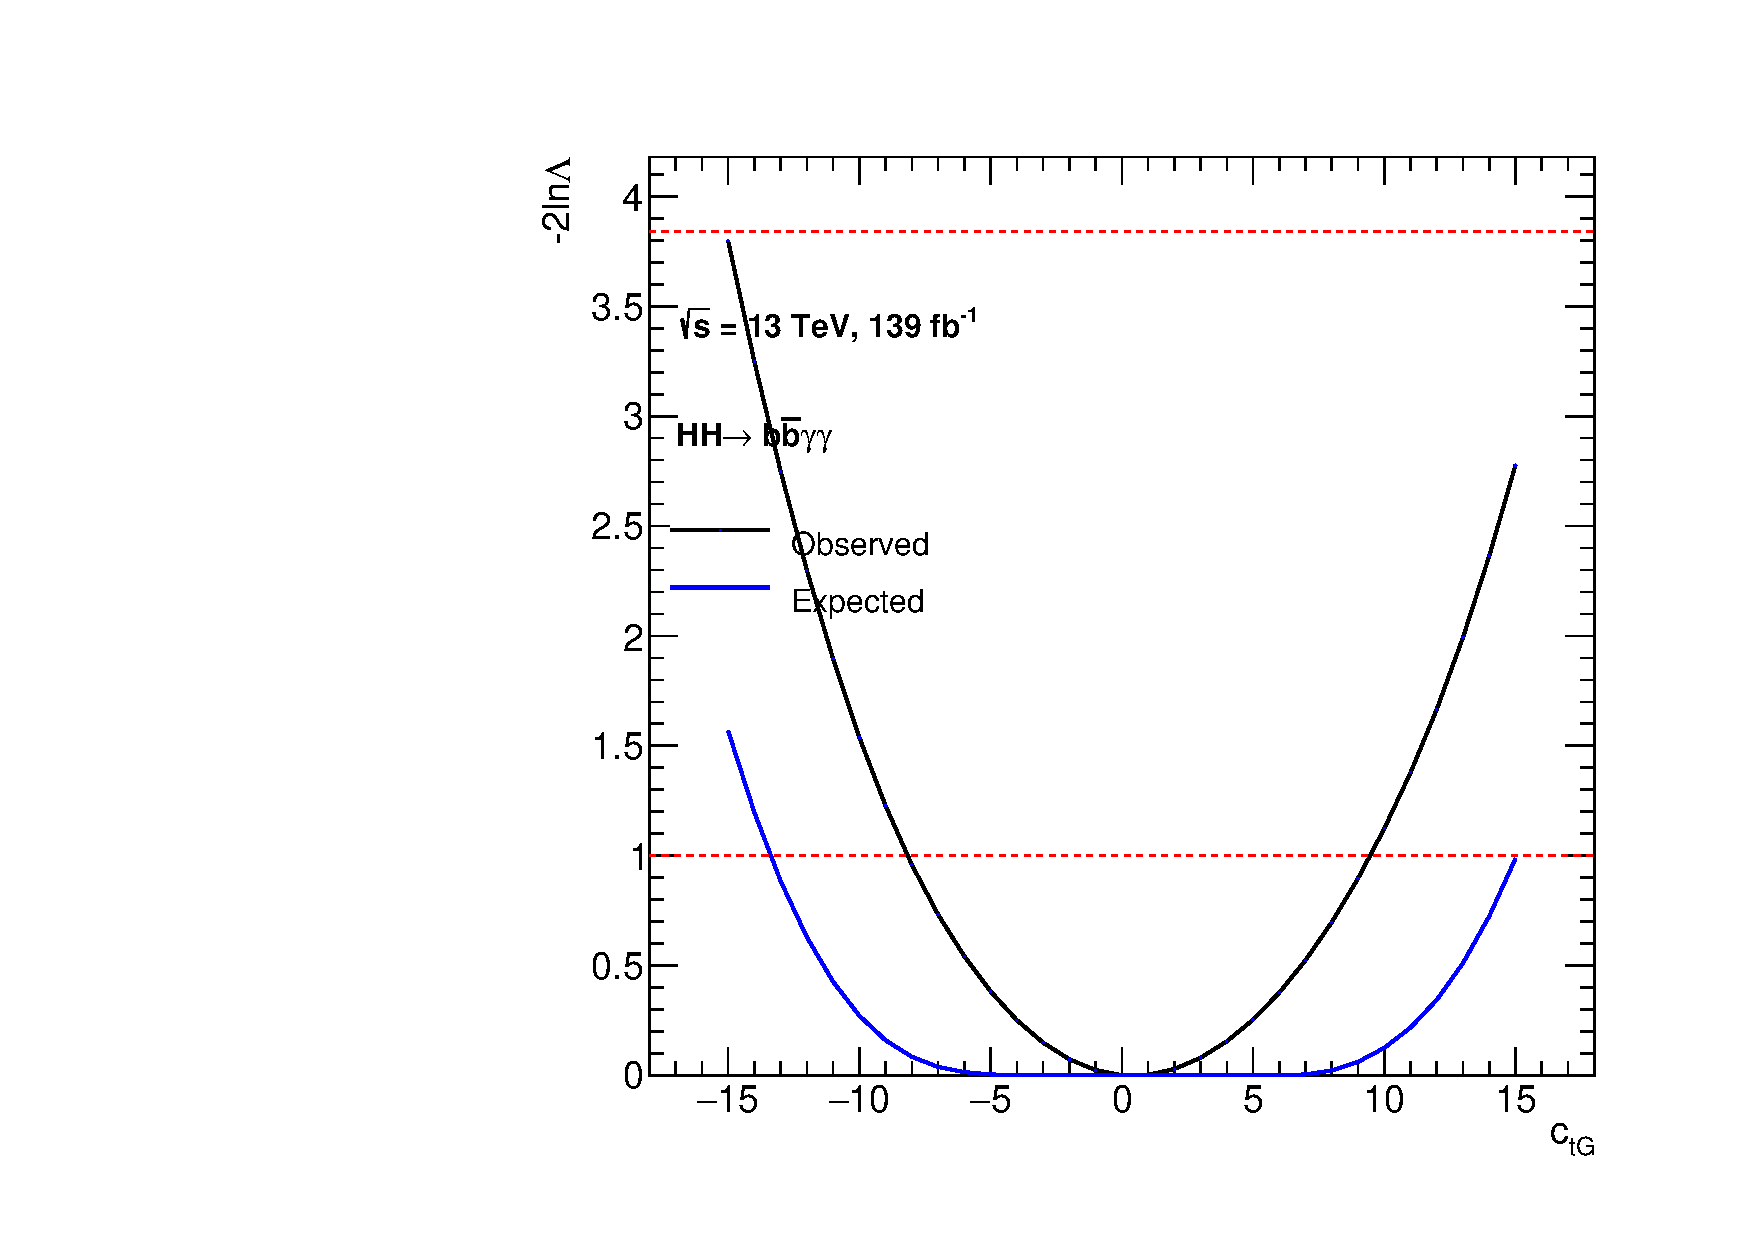
\includegraphics[width=0.5\textwidth]{BackUp/Part5/Img/subplot_NEW_ctG_Observed_Expected_1_cHkin_MG.pdf}}
\end{figure}

\end{columns}
\end{frame}

\begin{frame}{Sensitivity estimate}
    \begin{itemize}
        \item Looking at the eigenvectors of the inverse covariance matrix of Wilson coefficients 
            \begin{equation*}
                C^{-1}_{EFT} = P^T \cdot C^{-1}_{b\bar{b}\gamma\gamma} \cdot P
            \end{equation*}
        
         \item P is the parameterization matrix considering only linear terms. 
    \end{itemize}
   
    
    \begin{table}[]
    \centering
    \begin{tabular}{ll}
    \hline\hline
    Eigenvalue & Eigenvector \\
    \hline
    0.0523  &  - 0.582 $\cdot$ $c_{H}$ + 0.363 $\cdot$ $c_{H\square}$ - 0.456 $\cdot$ $c_{uH}$ + 0.567 $\cdot$ $c_{tG}$ \\ \hline
    0.0001  &  - 0.696 $\cdot$ $c_{H}$ + 0.182 $\cdot$ $c_{H\square}$ + 0.206 $\cdot$ $c_{uH}$ - 0.663 $\cdot$ $c_{tG}$ \\ \hline
    -0.0000 &  - 1.025 $\cdot$ $c_{H}$ - 1.947 $\cdot$ $c_{H\square}$ + 0.702 $\cdot$ $c_{uH}$ + 0.759 $\cdot$ $c_{tG}$ \\ \hline
    -0.0000 &  - 0.235 $\cdot$ $c_{H}$ - 0.006 $\cdot$ $c_{H\square}$ + 0.977 $\cdot$ $c_{uH}$ + 0.549 $\cdot$ $c_{tG}$ \\ \hline
   \hline
    \end{tabular}
\end{table}
\end{frame}

\begin{frame}{$c_{H}$ only}
\begin{figure}
    \centering
    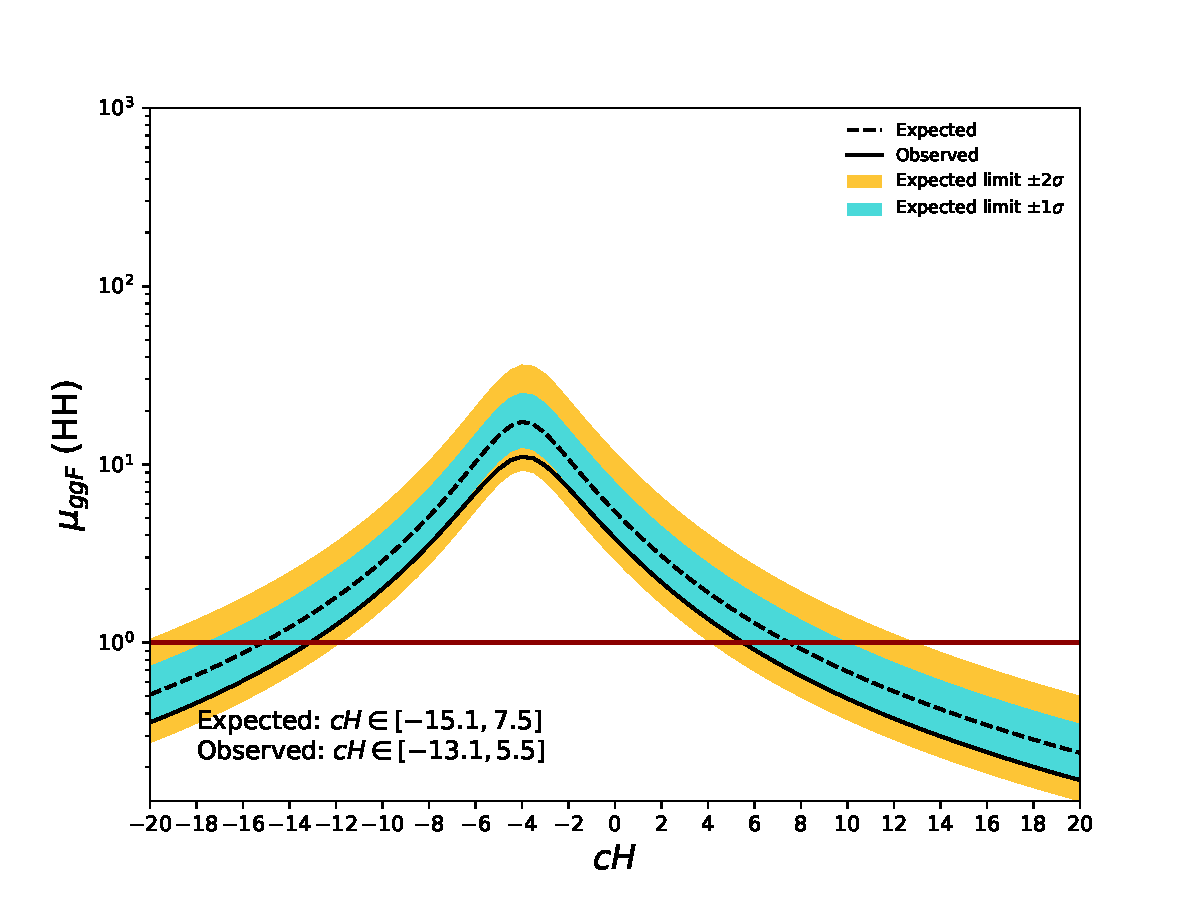
\includegraphics[width=0.6\textwidth]{BackUp/Part5/Img/cH_lambda.pdf}
\end{figure}
\end{frame}

\begin{frame}{$c_{H}$ vs $\kappa_{\lambda}$}
\begin{columns}
\column{0.5\textwidth}
\begin{figure}
    \centering
    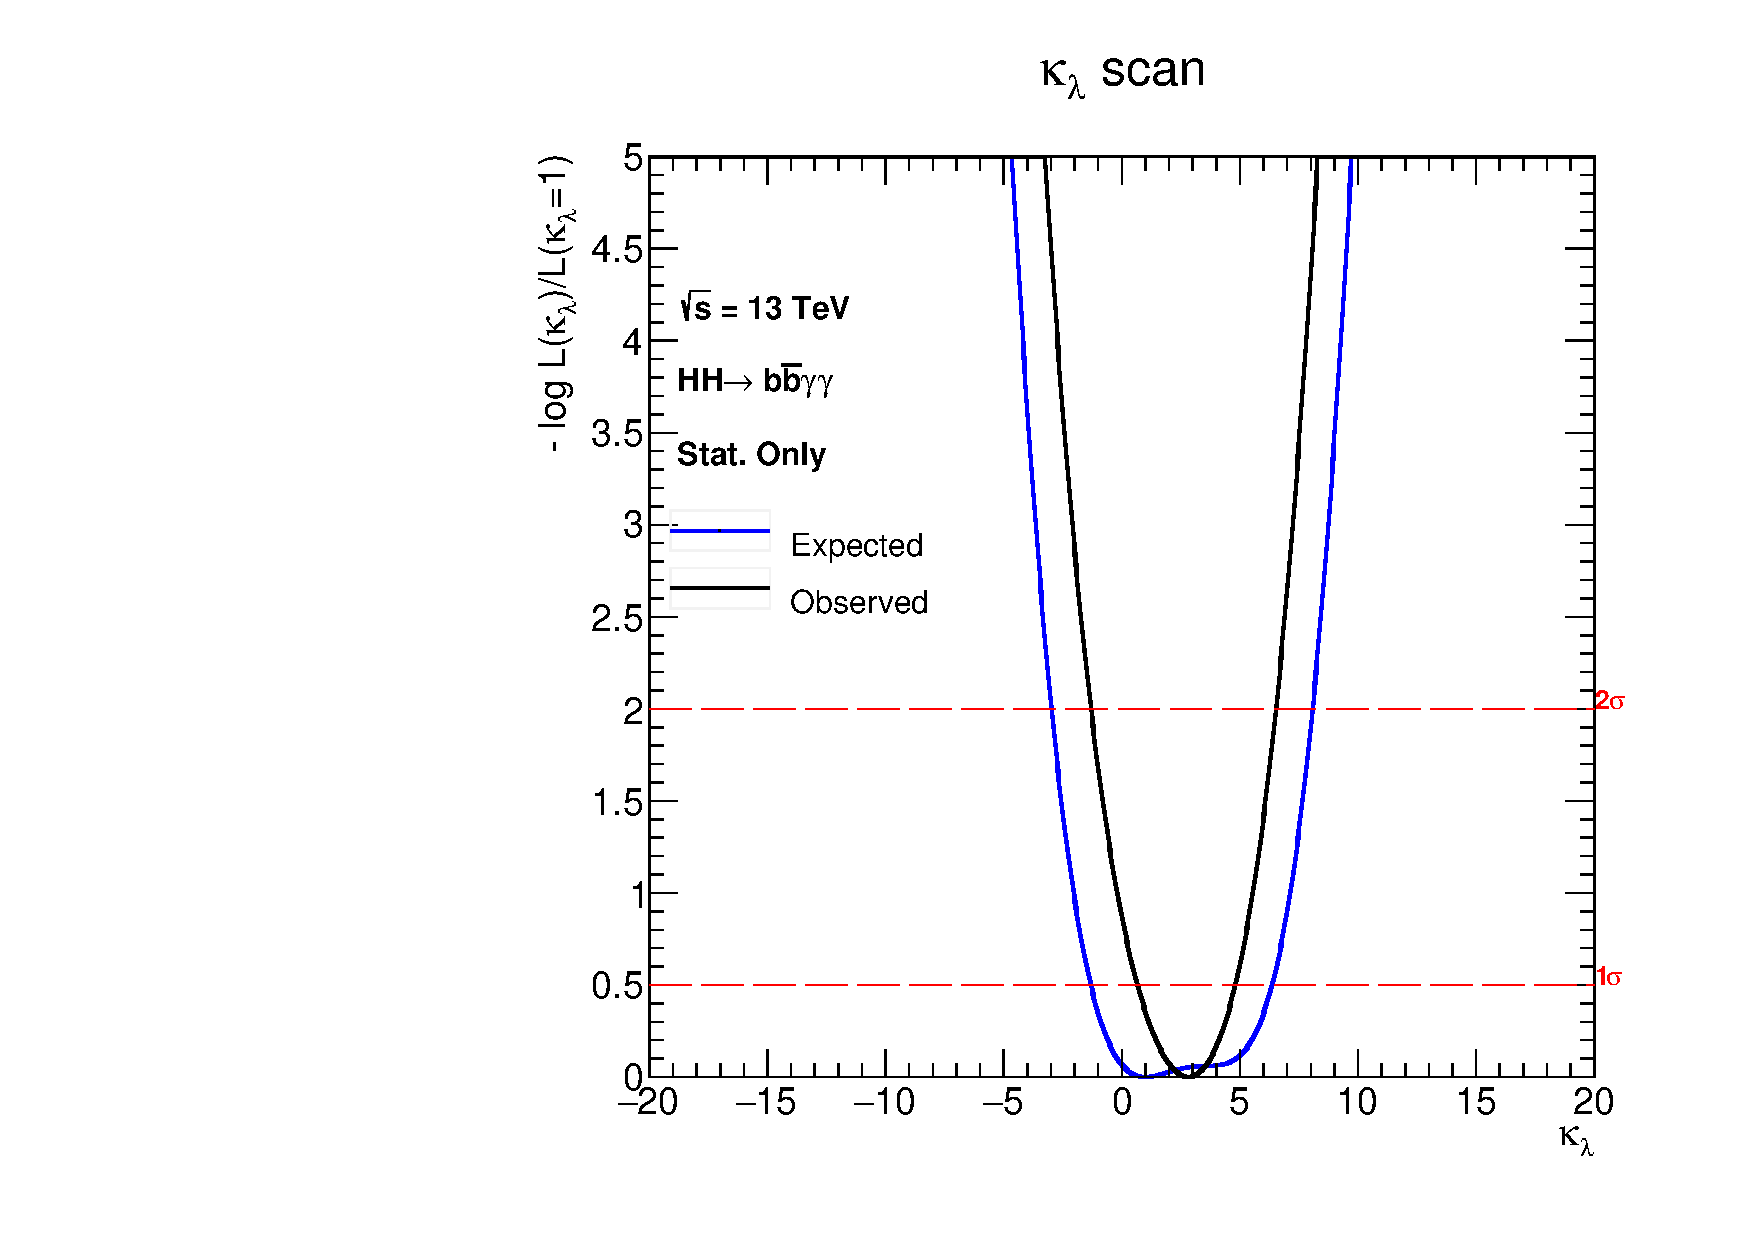
\includegraphics[width=1.\textwidth]{BackUp/Part5/Img/likelihood_subplot_kl.pdf}
\end{figure}
\column{0.5\textwidth}
\begin{figure}
    \centering
    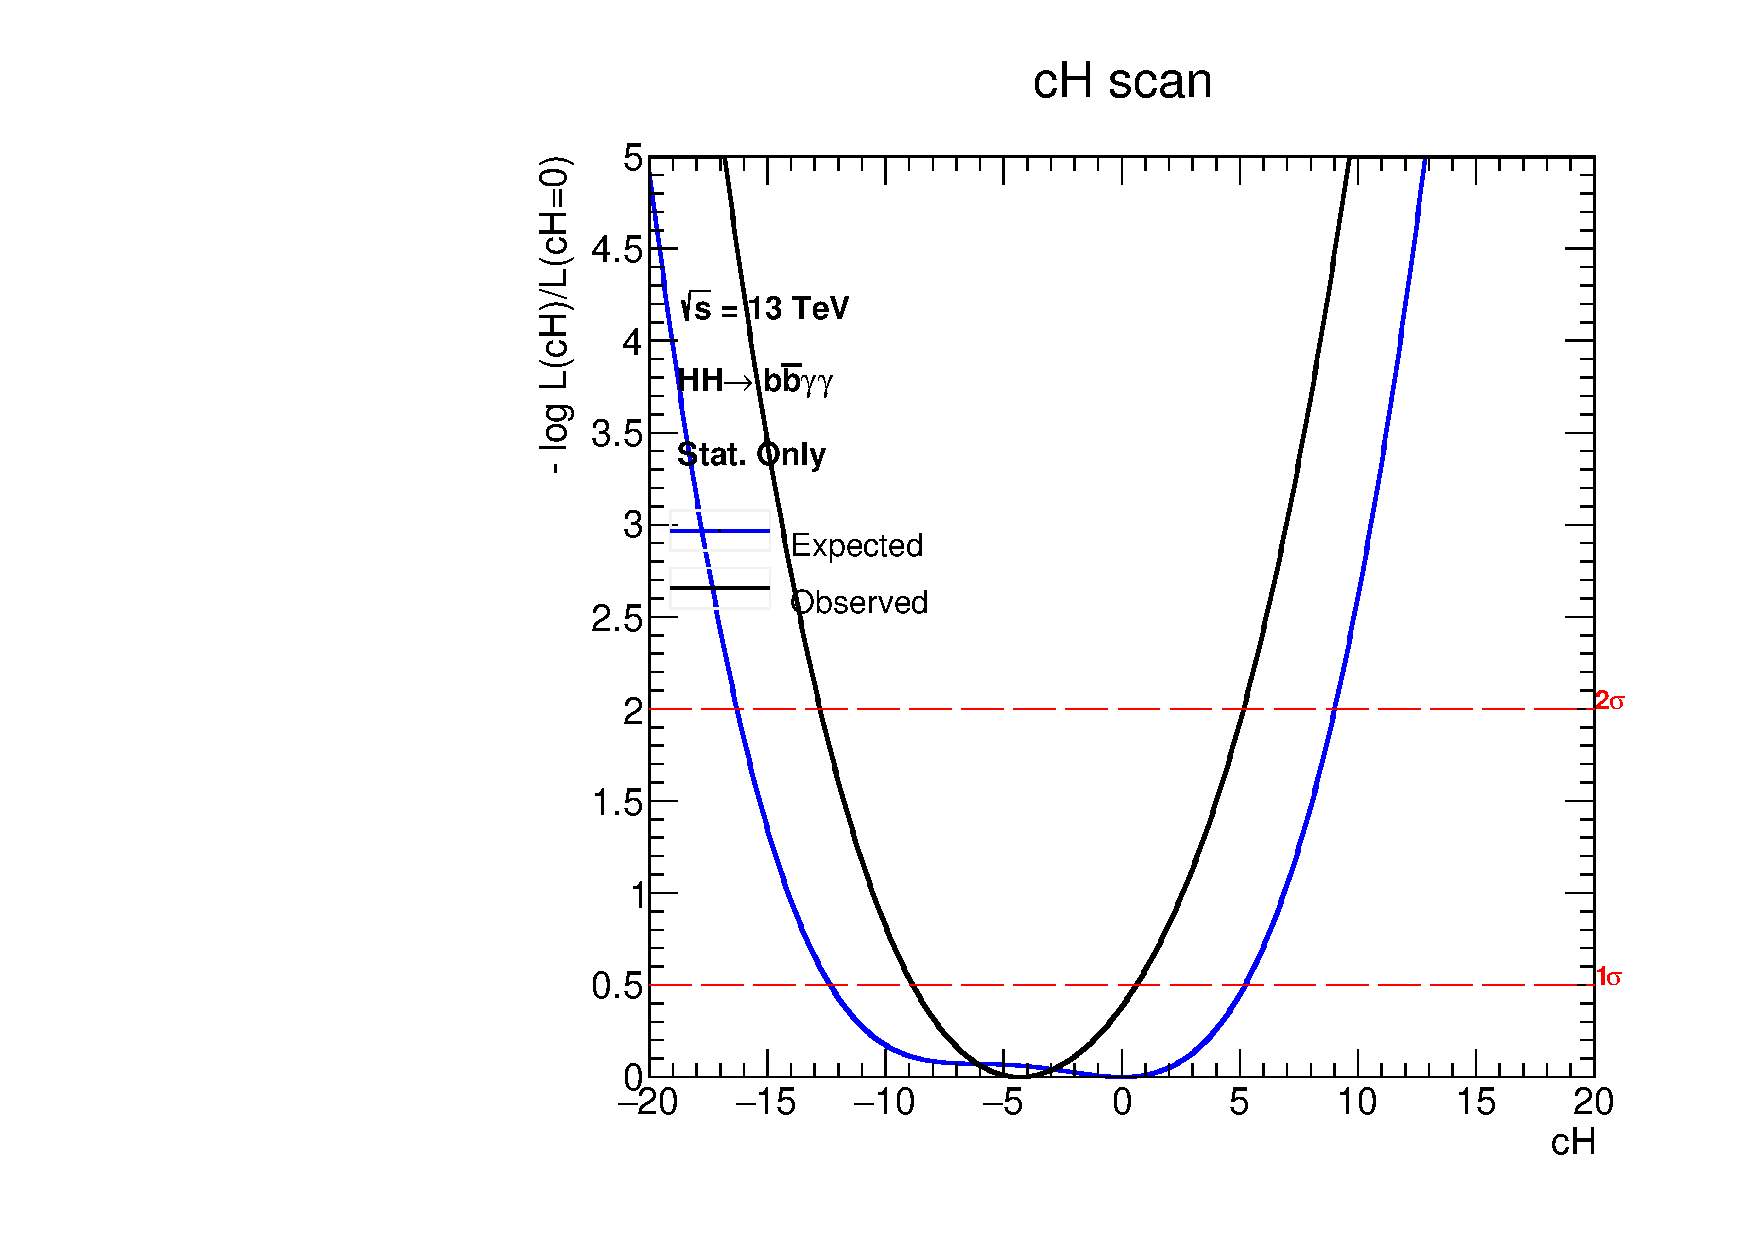
\includegraphics[width=1.\textwidth]{BackUp/Part5/Img/likelihood_subplot_cH.pdf}
\end{figure}
\end{columns}
\end{frame}

\begin{frame}{Linear vs Quadratic}

\begin{figure}
    \centering
    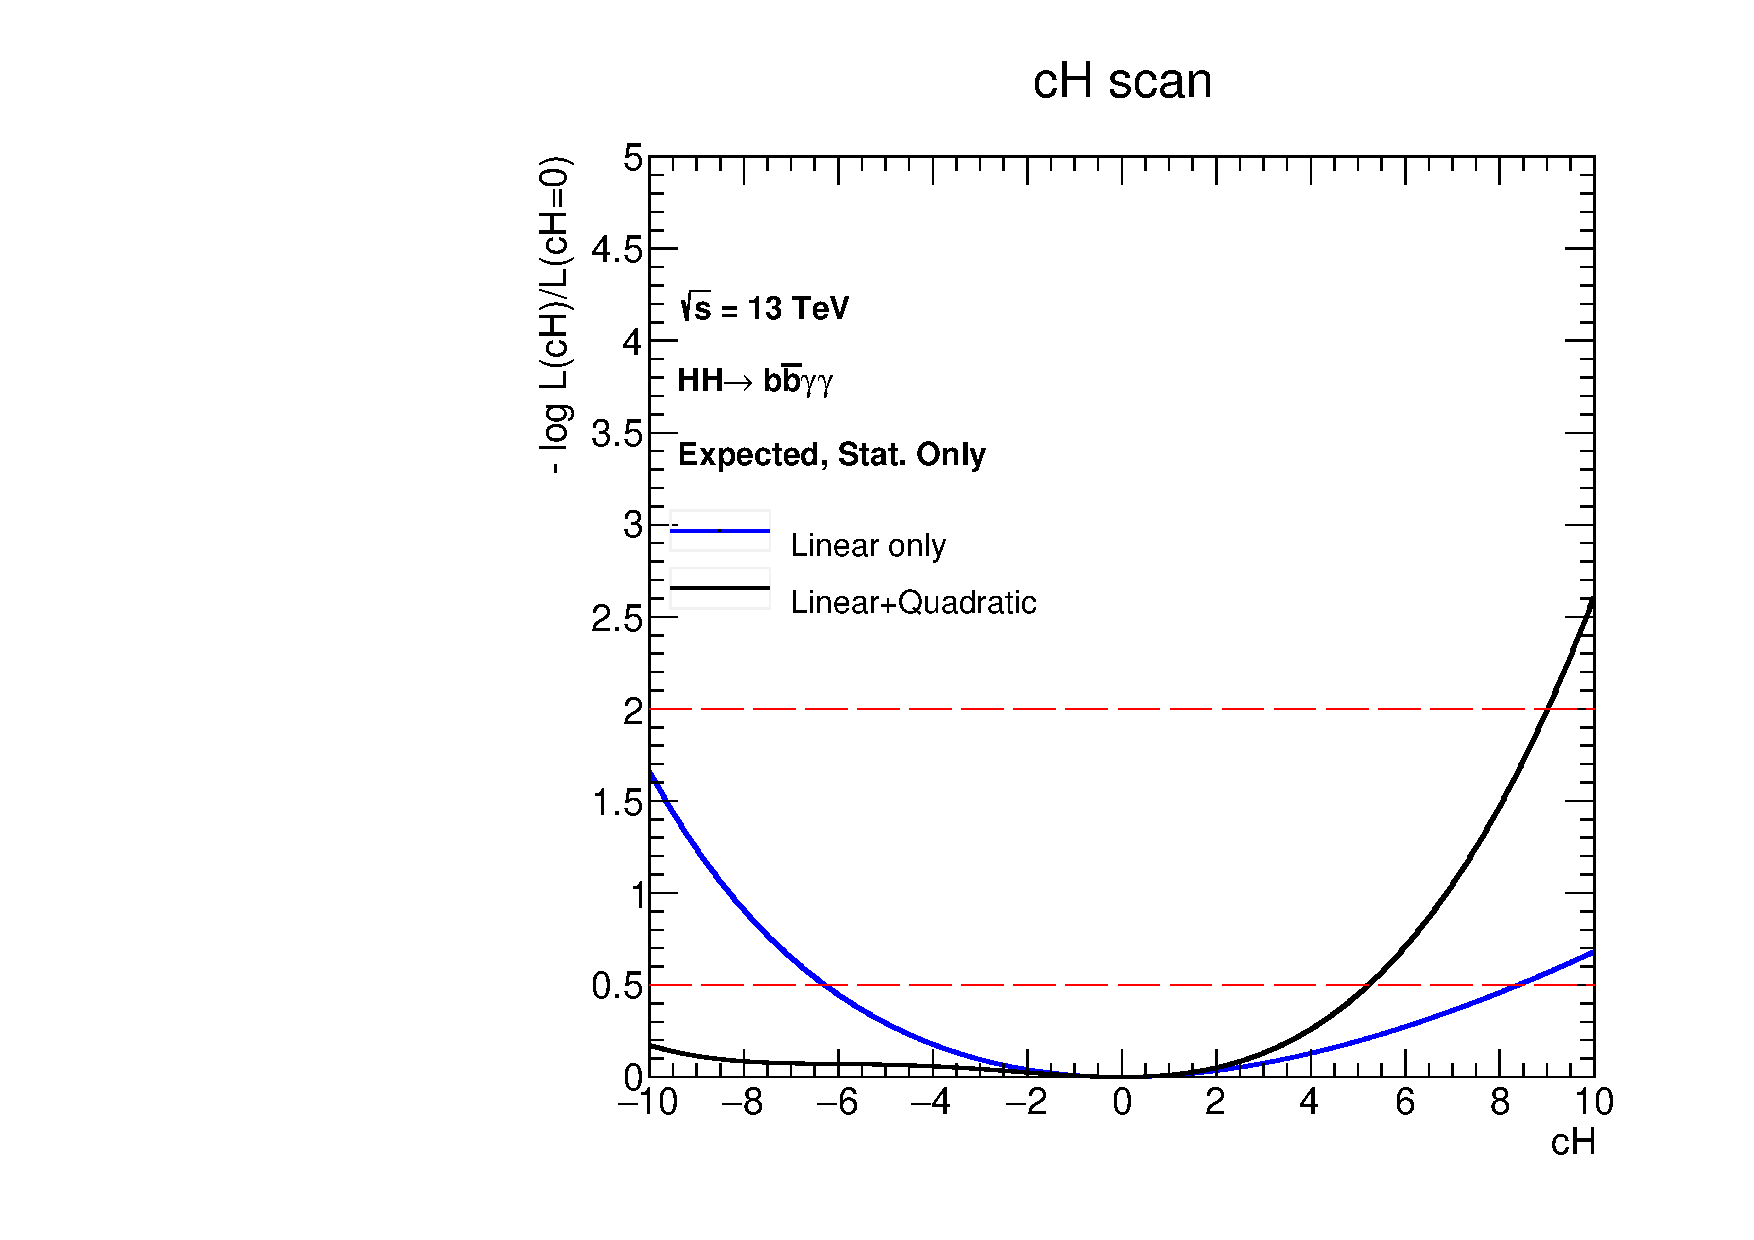
\includegraphics[width=0.5\textwidth]{BackUp/Part5/Img/likelihood_subplot_cp_lin_vs_quad_Exp.pdf}
\end{figure}
    
\end{frame}


